\documentclass[12pt]{article}

\usepackage{sbc-template}
\usepackage{graphicx,url}
\usepackage[utf8]{inputenc}
%\usepackage[brazil]{babel}
%\usepackage[latin1]{inputenc}  

     
\sloppy

\title{Guia para o uso do Geonode}

\author{NDS\inst{1}}


\address{
  NDS
\nextinstitute
  CPRM
\email{\{cprm,nds\}@sgb.gov.br}
}

\begin{document} 

\maketitle


\section{Introdução}

Este documento define procedimentos a serem utilizados para a carga de arquivos
e metadados no ambiente Geonode do SGB.

\section{Acesso} \label{sec:firstpage}

Para carregar arquivos no sistema Geonode, o usuário deve estar conectado em
uma conta com permissão para a carga. Para isso o usuário deve seguir o link na
parte superior direita da página para a tela de login e inserir suas
credenciais (ref{fig:login}).

\begin{figure}[h]
  \centering
  \includegraphics[width=\textwidth, keepaspectratio]{img/login.pdf}
  \caption{Caminho para a inserir as credenciais de login, em vermelho o link para acessar a página de login.}
  \label{fig:login}
\end{figure}


\section{Dados}

Com o acesso ao usuário com permissões para carga será possível visualizar o
menu de "Dados" no canto superior esquerda da página (Figura
\ref{fig:upload}.1). Duas opções estão disponíveis: datasets e documentos.
Datasets se referem aos arquivos de cunho de representação geoespacial
(shapefiles, geopackages, geojson, geotiff e outros) e documentos se referem
aos demais arquivos de registro de dados (pdf, jpeg, log, csv, zip e outros).

Após acessar o menu "Dados-Datasets" ou "Dados-Documentos" será possível
carregar novos dados utilizando o botão "Adicionar Recurso", no canto superior
direito da página (Figura \ref{fig:upload}.2). Em uma nova página o usuário
poderá utilizar o recurso de arrastar e soltar ou o botão de selecionar
arquivos no canto esquerdo da página (Figura \ref{fig:upload}.3), é possível
carregar mais de um arquivo durante este processo. Com os arquivos devidamente
selecionados o botão de "Upload" estará disponível para prosseguir o
carregamento (Figura \ref{fig:upload}.4). 

\textbf{Atenção, no caso de shapefiles será necessário que todos os seus
componentes sejam selecionados ou que todos os componentes sejam comprimidos em
um arquivo zip.}

Ao concluir o upload o usuário será redirecionado para uma página listando
todos os arquivos carregados. Ao clicar no nome do arquivo o usuário poderá
acessar sua página de detalhamento (Figura \ref{fig:upload}.5). O mesmo pode
ser feito através do menu "Dados" acessado anteriormente, clicando na imagem de
apresentação do dado e em seguida em visualizar.

Na página de detalhamento do dado é possível visualizar, filtrar e editar os
dados geoespaciais.

\begin{figure}[h]
  \centering
  \includegraphics[width=\textwidth, keepaspectratio]{img/upload.pdf}
  \caption{Fluxo para o upload de dados no Geonode.}
  \label{fig:upload}
\end{figure}

\section{Metadados}

Na página de detalhamento de um dado é possível editar seus metadados
através do menu "Editar-Editar Metadados"

Na página de edição de metadados o usuário pode alterar todos os aspectos do
metadado através de um formulário. A medida que os campos são completos uma
barra de progresso é atualizada. 

AQUI VAI UMA ESPECIFICAÇÃO SOBRE CADA METADADO?

\section{Mapas}

No menu Mapas na aba superior da página do Geonode é possível consultar os
mapas existentes e criar novos mapas. Usando o botão "Adicionar recursos" na
parte superior direita da página e em seguida "Criar mapa" é possível criar um
mapa a partir dos dados inseridos no Geonode.

\section{Carga de Bancos de Dados}

\subsection{Credenciais}
Para realizar a carga de Bancos de Dados, é necessário o acesso de um usuário
com permissão de administrador no ambiente Geonode. Através do menu do usuário
na parte superior direita acesse o Geoserver. Na página do Geoserver clique na
aba de login na parte superior, a página irá garantir acesso de administrador,
caso o contrário realize o login usando as credenciais de administrador do
Geoserver.

\subsection{Stores}
Uma vez conectado com acesso de administrador na página do Geoserver. Entre na
aba "Store" na lateral esquerda da página e em seguida crie um novo Store.
Selecione a opção "PostGISDatabase". Um formulário deverá ser preenchido para a
criação de um novo Store, atente para os parâmetros host e port que devem ser
os parâmetros do banco de dados na mesma localização do Geonode. \textbf{O
parâmetro workspace deve ser Geonode}. Os parâmetros de usuário e senha devem
ser os mesmos utilizados pelo Geonode no Postgres. Ao finalizar a criação de um
novo store a página irá te redirecionar para a aba "New Layer".

\subsection{Layers}
Dentro da aba "New Layer", acessando pelo menu lateral esquerdo ou
redirecionado pela aba Store, estarão disponíveis os feature classes presentes
no banco de dados em uma tabela. Ao clicar no botão "Publish" a página será
redirecionada para um formulário com informações sobre a feature class já
preenchidas. O usuário deve verificar se o sistema de referência está
corretamente detectado pelo Geoserver, em caso negativo o sistema deverá ser
explicitado de acordo com o código EPSG. Com o sistema devidaemente
identificado as extensões do feature class devem ser definidas por meio do
botão "Compute from data". Feito isso, a layer pode ser salva e estará
disponível no Geoserver.

\subsection{Django}
Para que as mudanças no Geoserver sejam visíveis no Geonode é necessário
atualizar as layers as quais o Django tem acesso. Para isso, é necessário
utilizar o script "manage.py" usando o argumento "updatelayers" dentro do
container que hospeda a instância do Django. Uma vez com o terminal dentro da
instância do Django basta utilizar o seguinte comando: 

python manage.py updatelayers

Após sua execução será informado se o Django obteve sucesso no upload das novas
layers e em caso positivo será possível visualiza-las através do Geonode.

\bibliographystyle{sbc}
\bibliography{sbc-template}

\end{document}
